\subsection{Prototipo}
\label{subsec:prototipo}

El desarrollo del prototipo de la lanzadera electromagnética constituye una etapa crucial en la validación del modelo teórico y las diferentes simulaciones realizadas en fases previas. Esta sección se centra en el diseño y construcción de un dispositivo funcional que permita la evaluación práctica de los conceptos estudiados y la obtención de datos experimentales que respalden las predicciones teóricas.

El objetivo principal del prototipo es proporcionar una plataforma experimental (a la que se le llamará \textit{banco de pruebas}) que permita comprobar la efectividad de las configuraciones propuestas y realizar ajustes basados en observaciones empíricas. No se pretende construir una lanzadera electromagnética como la de la figura \ref{fig:prototipolanzadera}, sino más bien un prototipo modular que sea fácilmente modificable para poder probar diferentes configuraciones de bobina y alimentación. Una de las partes más importantes del prototipo ha sido la implementación de un sistema de medición capaz de registrar con exactitud la velocidad y fuerza del proyectil.

El siguiente apartado detalla los pasos específicos seguidos en el desarrollo del prototipo, desde el montaje del banco de pruebas, el diseño del circuito electrónico y la construcción de la bobina, hasta el ensamblaje sistema completo. Cada uno de estos pasos ha conllevado más de una iteración hasta llegar al resultado final, que es lo que se va a detallar en esta sección. Sin embargo, en el Anexo II se puede encontrar el proceso más detallado.

FOTO DEL PROTOTIPO FINAL

\newpage

\subsubsection{Materiales}
\label{subsub:materiales}
Para el montaje del prototipo, se utilizaron perfiles técnicos estructurales de aluminio como el que se presenta en la siguiente figura:

\textbf{FIGURA DE LOS PERFILES DE ALUMINIO}

La ventaja de utilizar estos perfiles es que se puede modificar de manera muy sencilla la distribución de las diferentes partes del montaje, las cuales consisten en: dos parejas de perfiles en \textbf{T} que sirven de apoyo para el resto de la estructura, un perfil inferior que es en el que se coloca la bobina y un perfil superior que es en el que se colocan los sensores de movimiento y el circuito electrónico.

\textbf{FIGURA DEL BANCO SOLO CON LOS PERFILES}

Se describirán con detalle los sensores de movimiento, las restricciones de la bobina y el circuito electrónico diseñado para el proyecto.

\subsubsection{Sensores de movimiento}
\label{subsub:sensoresmov}

Los sensores de movimiento utilizados para el proyecto tienen como objetivo proporcionar la velocidad a la que sale el vástago de la bobina. Los que se han empleado son sensores de carácter capacitivo, lo que significa que detectan la presencia de un objeto delante de ellos por el cambio de la capacidad con la superficie del sensor. Colocando dos de estos dispositivos a una distancia conocida \textit{x} y obteniendo la diferencia temporal \(\Delta t\) de activación de la señal mediante una placa arduino conectada al sistema, es trivial calcular la velocidad del vástago según la fórmula:

\[v_{vas}=\frac{x}{\Delta t}\]

Los sensores elegidos para llevar a cabo esta tarea son los \textbf{MODELO SENSORES}, los cuales tienen el siguiente esquema de conexión:

\begin{figure}[H]
    \centering
    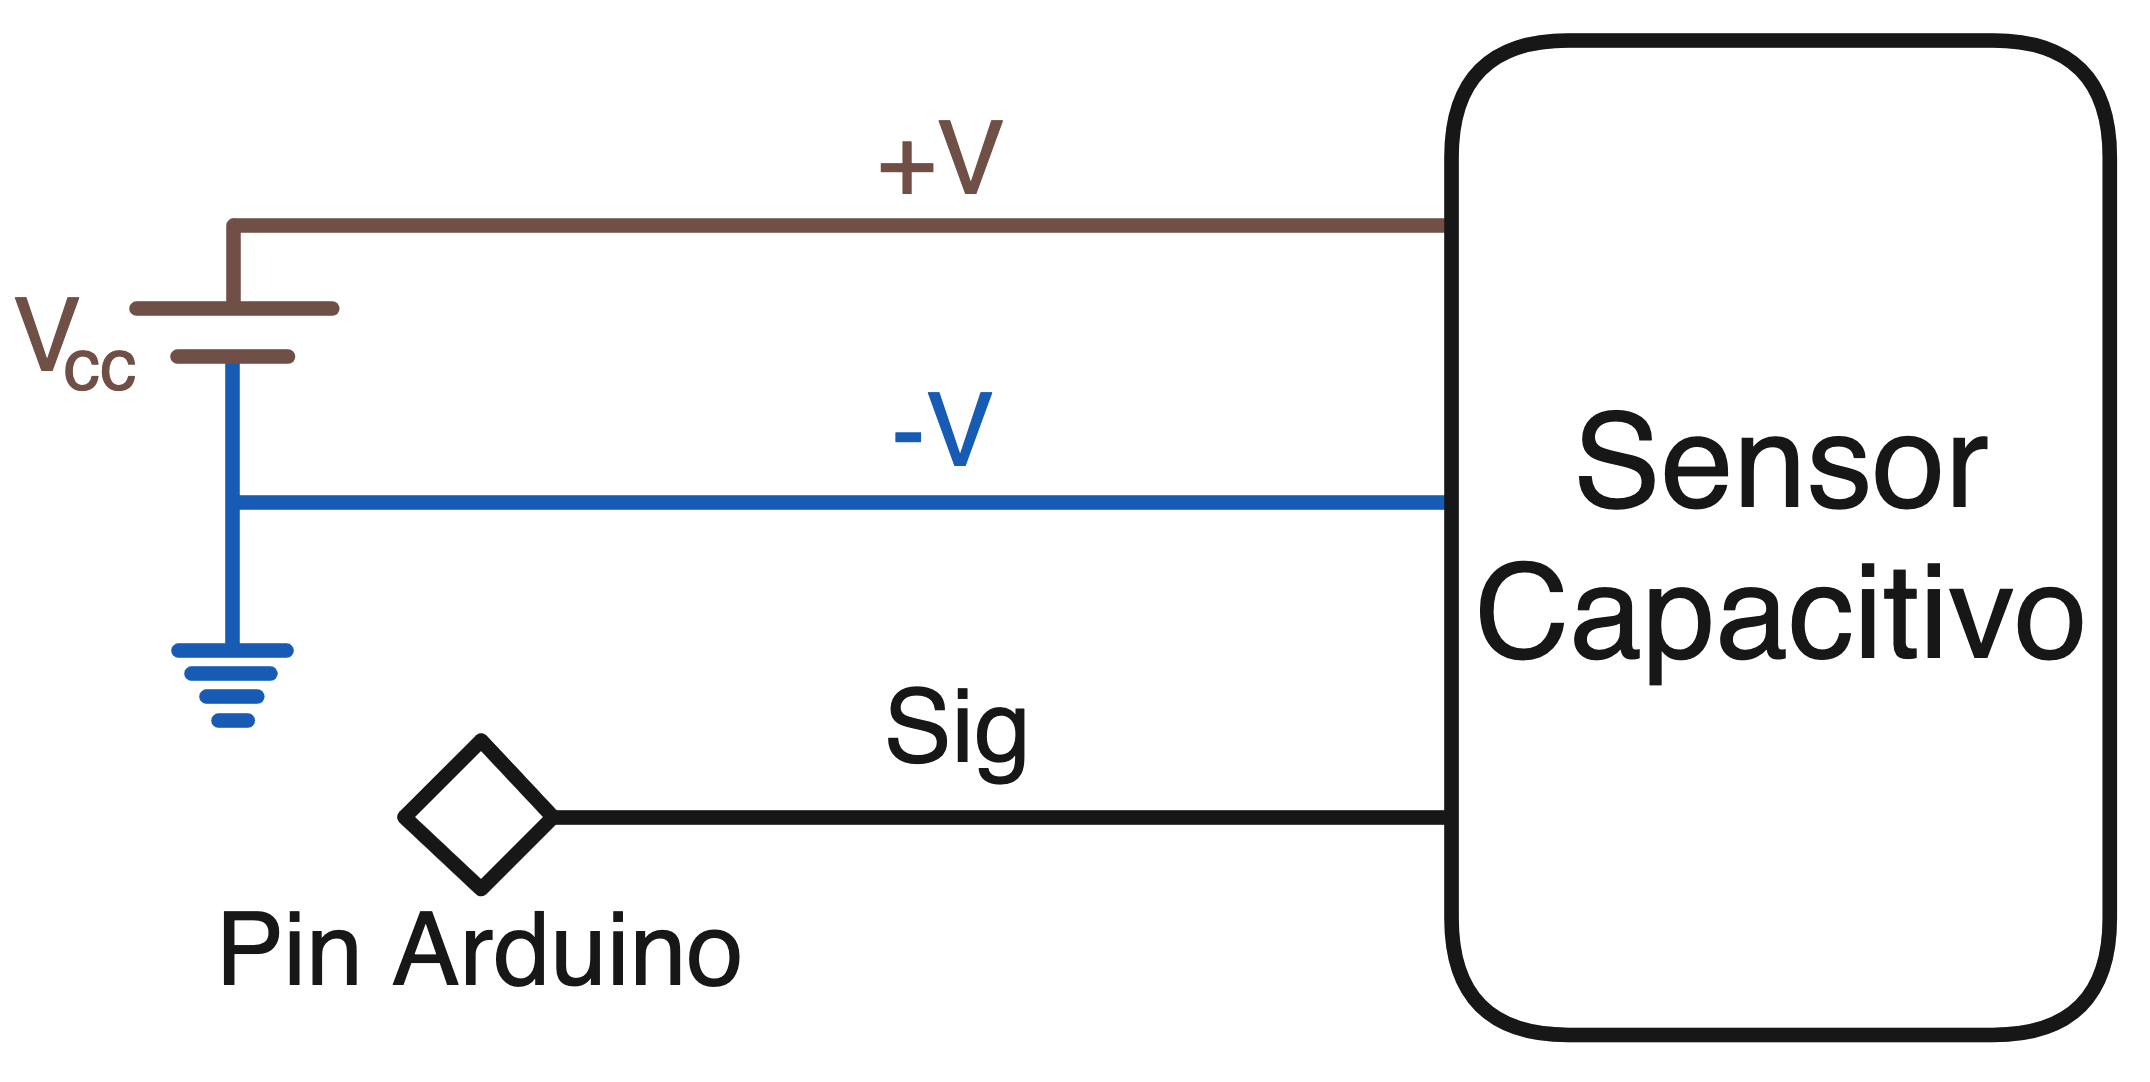
\includegraphics[width=10cm]{FigurasMemoria/esquemaSensor.png}
    \caption{Esquema conexiones del \textbf{MODELO SENSORES}. Elaboración propia.}
    \label{fig:esquemaSensor} %Para referenciar -> \ref{fig:figNum}
\end{figure}

La tensión de alimentación del sensor es de \(V_{cc}\in [6,~30]~V\), y la salida de la señal (tensión entre \textbf{SIG} y \textbf{GND}) es de \(V_{sig}=V_{cc}\). Esto es algo a tener en cuenta, pues la entrada de los puertos de arduino no puede superar los \(5~V\). Montando el prototipo, se decidió que el circuito electrónico iba a estar alimentado a \(15~V\), por lo que será necesario un divisor de tensiones para poder leer la señal de los sensores, el cual está detallado en el apartado de diseño del circuito \ref{subsub:circuito}.

\subsubsection{Circuito electrónico}
\label{subsub:circuito}
El diseño y desarrollo de la lanzadera electromagnética no solo requiere de la implementación de los componentes físicos de soporte, bobina y vástago, sino que también es esencial el diseño de un circuito electrónico que controle y optimice su funcionamiento. La precisión y eficiencia del dispositivo dependen en gran medida de la electrónica que lo acompaña. Durante el proceso de montaje del banco de pruebas, se han identificado dos etapas críticas de las cuales se debe encargar el circuito electrónico: la etapa de disparo y la etapa de medición.

\subsubsection*{Disparo}

Para el disparo, debemos indentificar dos momentos críticos, los de inicio y finalización de alimentación de la bobina para que el vástago adquiera inercia sin quedarse atascado en el campo magnético. Cuando se empezó el proyecto se pensó en realizar los disparos a mano apagando y encendiendo la fuente del solenoide, pero al realizar las simulaciones, se descubrió la imposibilidad de este método ya que la constante de tiempo (\(\tau\)) del sistema ronda los \(10^{-2}~s\) o \(10~ms\). Esto plantea un problema a la hora de disparar el vástago, pues debemos alimentar la bobina por un período de tiempo muy breve, lo cual es prácticamente imposible de hacer manualmente. Es necesario por ende diseñar de manera electrónica las órdenes de inicio y finalización del disparo del vástago.

El inicio del disparo es trivial, y tratará de un interruptor conectado a la placa arduino. Esta detectará la pulsación del interruptor y mandará la orden de disparo a través del mecanismo correspondiente.

\begin{figure}[H]
    \centering
    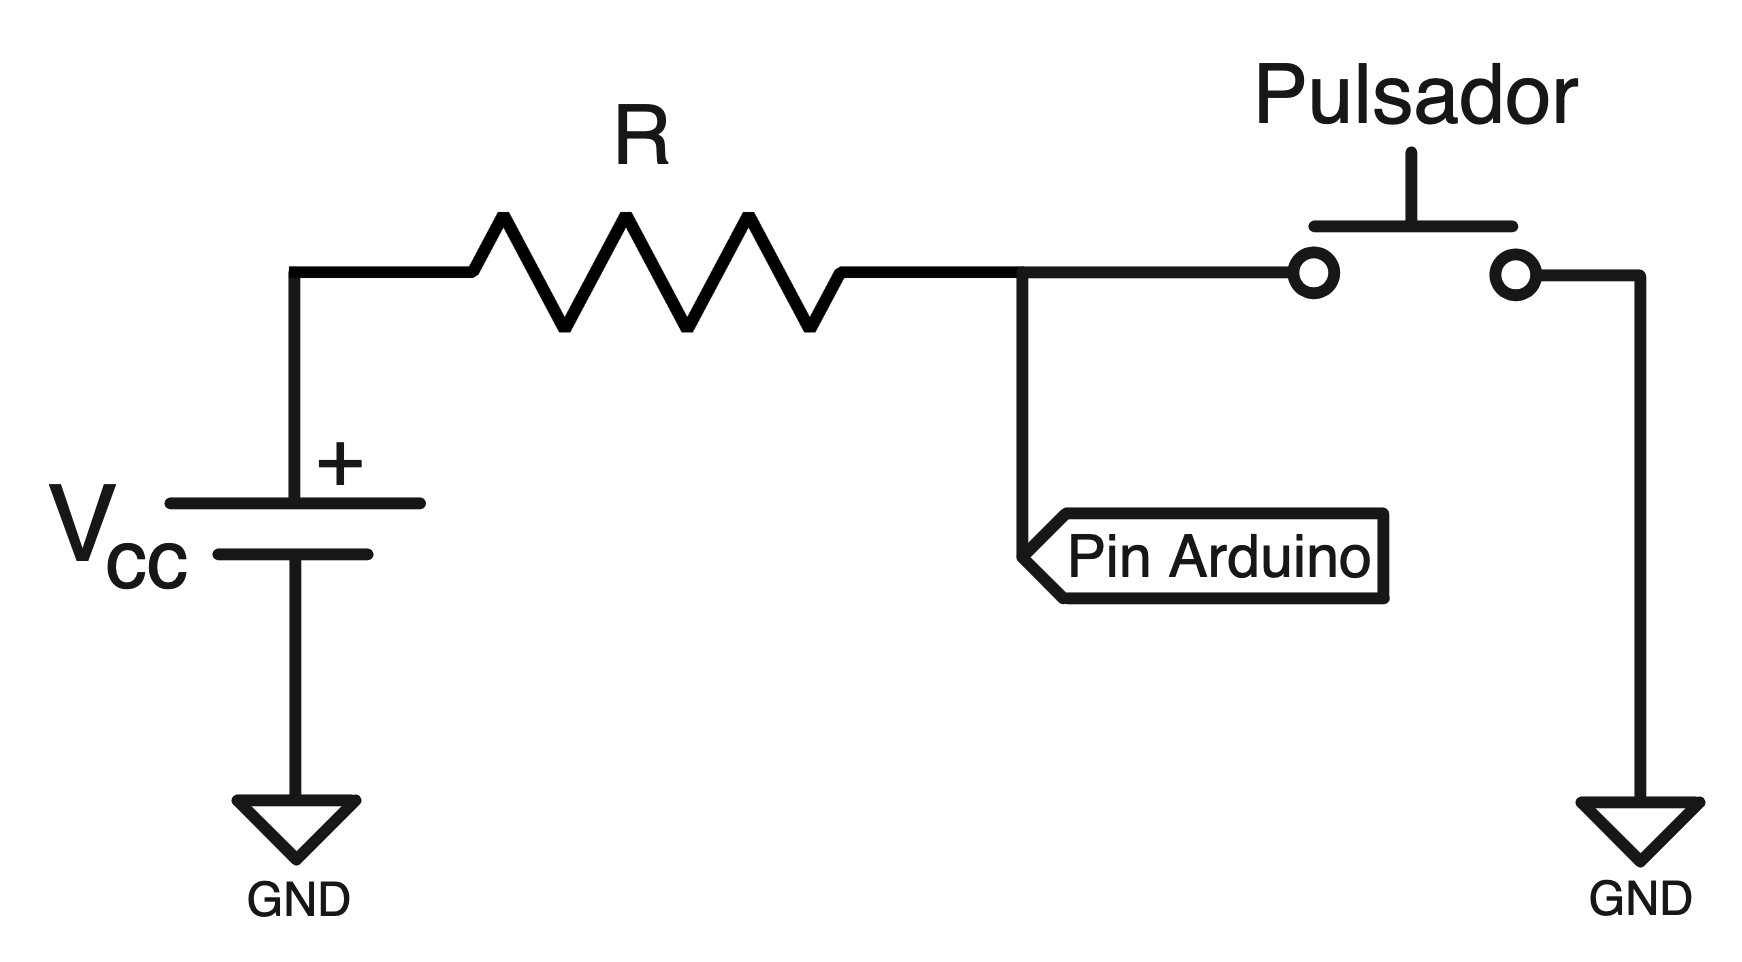
\includegraphics[width=4cm]{FigurasMemoria/conexionInterruptor.png}
    \caption{Conexión del interrupor de disparo. Elaboración propia.}
    \label{fig:conexionInterruptor} %Para referenciar -> \ref{fig:figNum}
\end{figure}

Por otro lado, la finalización del disparo es más compleja. Es necesario dejar de alimentar la bobina antes de que su centro esté alineado con el del vástago, ya que de lo contrario, este seguirá siendo atraído por el campo magnético y no adquirirá la inercia necesaria para que su movimiento continúe. Para lograr esto, se va a aprovechar el hecho de que por diseño \(l_{fe}~\geq~h_c\), colocando uno de los sensores de movimiento justo a la salida de la bobina. Esto permitirá obtener la señal de detección del primer sensor en el momento preciso en que sea necesario cortar la alimentación del solenoide, garantizando que el vástago adquiera la inercia adecuada para su desplazamiento.

\begin{figure}[H]
    \centering
    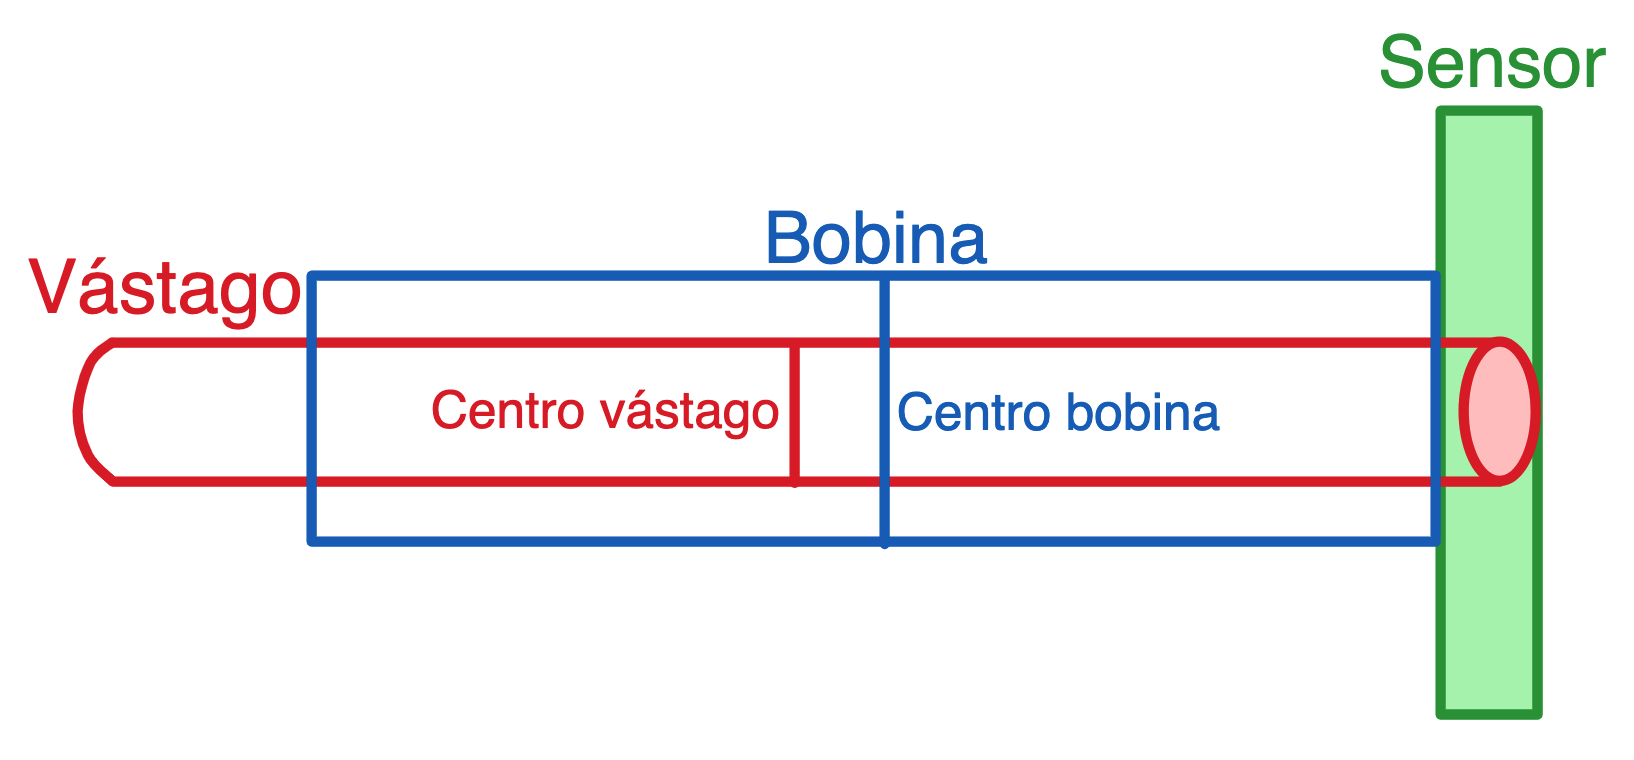
\includegraphics[width=10cm]{FigurasMemoria/esquemaJustDisparo.png}
    \caption{Colocación del sensor. Elaboración propia.}
    \label{fig:esquemaJustDisparo} %Para referenciar -> \ref{fig:figNum}
\end{figure}

La señal generada por el sensor de movimiento será enviada a un Arduino, que la procesará y activará un relé de potencia de estado sólido conectado a uno de sus pines. Este relé estará conectado a una fuente de corriente y será responsable de interrumpir la alimentación de la bobina en el momento adecuado. El uso de un relé de estado sólido asegura una conmutación rápida y precisa, eliminando la alimentación de la bobina de manera efectiva y asegurando el correcto funcionamiento del sistema de disparo.
 
\subsubsection{Bobina}
\label{subsub:bobina}

Los solenoides que se prueben en el prototipo deben de cumplir las siguientes especificaciones:


\begin{itemize}
    \item \(0.5\leq h_{c} \leq XX\): la longitud máxima de la bobina está delimitada por la longitud del perfil menos un espacio mínimo entre sensores.
\end{itemize}